\documentclass[tikz,10pt,border=0.5cm]{standalone}

\usetikzlibrary{decorations.pathreplacing}

\begin{document}
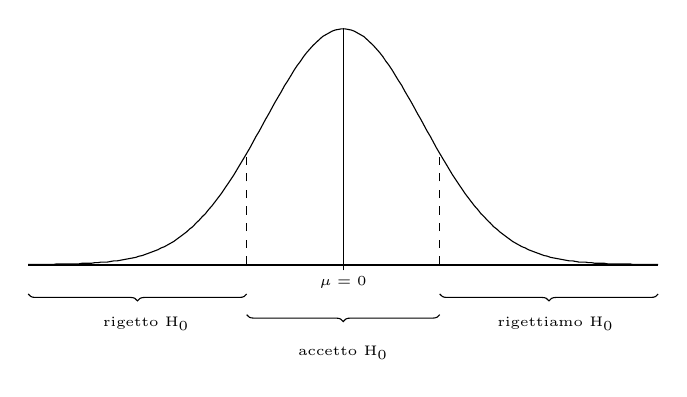
\begin{tikzpicture}[x=1cm,y=7.5cm]

\draw(-4,-0.001)--(4,-0.001);

\draw (-4.0,0.0) -- (-3.96,0.0) -- (-3.92,0.0) -- (-3.879,0.0) -- (-3.839,0.0) -- (-3.799,0.0) -- (-3.759,0.0) -- (-3.719,0.0) -- (-3.678,0.0) -- (-3.638,0.001) -- (-3.598,0.001) -- (-3.558,0.001) -- (-3.518,0.001) -- (-3.477,0.001) -- (-3.437,0.001) -- (-3.397,0.001) -- (-3.357,0.001) -- (-3.317,0.002) -- (-3.276,0.002) -- (-3.236,0.002) -- (-3.196,0.002) -- (-3.156,0.003) -- (-3.116,0.003) -- (-3.075,0.004) -- (-3.035,0.004) -- (-2.995,0.004) -- (-2.955,0.005) -- (-2.915,0.006) -- (-2.874,0.006) -- (-2.834,0.007) -- (-2.794,0.008) -- (-2.754,0.009) -- (-2.714,0.01) -- (-2.673,0.011) -- (-2.633,0.012) -- (-2.593,0.014) -- (-2.553,0.015) -- (-2.513,0.017) -- (-2.472,0.019) -- (-2.432,0.021) -- (-2.392,0.023) -- (-2.352,0.025) -- (-2.312,0.028) -- (-2.271,0.03) -- (-2.231,0.033) -- (-2.191,0.036) -- (-2.151,0.039) -- (-2.111,0.043) -- (-2.07,0.047) -- (-2.03,0.051) -- (-1.99,0.055) -- (-1.95,0.06) -- (-1.91,0.064) -- (-1.869,0.07) -- (-1.829,0.075) -- (-1.789,0.081) -- (-1.749,0.086) -- (-1.709,0.093) -- (-1.668,0.099) -- (-1.628,0.106) -- (-1.588,0.113) -- (-1.548,0.12) -- (-1.508,0.128) -- (-1.467,0.136) -- (-1.427,0.144) -- (-1.387,0.152) -- (-1.347,0.161) -- (-1.307,0.17) -- (-1.266,0.179) -- (-1.226,0.188) -- (-1.186,0.197) -- (-1.146,0.207) -- (-1.106,0.217) -- (-1.065,0.226) -- (-1.025,0.236) -- (-0.985,0.246) -- (-0.945,0.255) -- (-0.905,0.265) -- (-0.864,0.275) -- (-0.824,0.284) -- (-0.784,0.293) -- (-0.744,0.303) -- (-0.704,0.311) -- (-0.663,0.32) -- (-0.623,0.329) -- (-0.583,0.337) -- (-0.543,0.344) -- (-0.503,0.352) -- (-0.462,0.359) -- (-0.422,0.365) -- (-0.382,0.371) -- (-0.342,0.376) -- (-0.302,0.381) -- (-0.261,0.386) -- (-0.221,0.389) -- (-0.181,0.392) -- (-0.141,0.395) -- (-0.101,0.397) -- (-0.06,0.398) -- (-0.02,0.399) -- (0.02,0.399) -- (0.06,0.398) -- (0.101,0.397) -- (0.141,0.395) -- (0.181,0.392) -- (0.221,0.389) -- (0.261,0.386) -- (0.302,0.381) -- (0.342,0.376) -- (0.382,0.371) -- (0.422,0.365) -- (0.462,0.359) -- (0.503,0.352) -- (0.543,0.344) -- (0.583,0.337) -- (0.623,0.329) -- (0.663,0.32) -- (0.704,0.311) -- (0.744,0.303) -- (0.784,0.293) -- (0.824,0.284) -- (0.864,0.275) -- (0.905,0.265) -- (0.945,0.255) -- (0.985,0.246) -- (1.025,0.236) -- (1.065,0.226) -- (1.106,0.217) -- (1.146,0.207) -- (1.186,0.197) -- (1.226,0.188) -- (1.266,0.179) -- (1.307,0.17) -- (1.347,0.161) -- (1.387,0.152) -- (1.427,0.144) -- (1.467,0.136) -- (1.508,0.128) -- (1.548,0.12) -- (1.588,0.113) -- (1.628,0.106) -- (1.668,0.099) -- (1.709,0.093) -- (1.749,0.086) -- (1.789,0.081) -- (1.829,0.075) -- (1.869,0.07) -- (1.91,0.064) -- (1.95,0.06) -- (1.99,0.055) -- (2.03,0.051) -- (2.07,0.047) -- (2.111,0.043) -- (2.151,0.039) -- (2.191,0.036) -- (2.231,0.033) -- (2.271,0.03) -- (2.312,0.028) -- (2.352,0.025) -- (2.392,0.023) -- (2.432,0.021) -- (2.472,0.019) -- (2.513,0.017) -- (2.553,0.015) -- (2.593,0.014) -- (2.633,0.012) -- (2.673,0.011) -- (2.714,0.01) -- (2.754,0.009) -- (2.794,0.008) -- (2.834,0.007) -- (2.874,0.006) -- (2.915,0.006) -- (2.955,0.005) -- (2.995,0.004) -- (3.035,0.004) -- (3.075,0.004) -- (3.116,0.003) -- (3.156,0.003) -- (3.196,0.002) -- (3.236,0.002) -- (3.276,0.002) -- (3.317,0.002) -- (3.357,0.001) -- (3.397,0.001) -- (3.437,0.001) -- (3.477,0.001) -- (3.518,0.001) -- (3.558,0.001) -- (3.598,0.001) -- (3.638,0.001) -- (3.678,0.0) -- (3.719,0.0) -- (3.759,0.0) -- (3.799,0.0) -- (3.839,0.0) -- (3.879,0.0) -- (3.92,0.0) -- (3.96,0.0) -- (4.0,0.0) ;

\draw[](0,-0.01)--(0,0.01);
\draw[](0,0)--(0,0.4);

\draw[dashed] (-1.226,0) -- (-1.226,0.188) ;
\draw[dashed] (1.226,0) -- (1.226,0.188) ;

\node (mu) at (0,-0.03){\tiny$\mu=0$};

\draw [decorate, decoration = {brace,mirror}] (-4,-0.05) --  (-1.226,-0.05);
\draw [decorate, decoration = {brace,mirror}] (1.226,-0.05) --  (4,-0.05);

\draw [decorate, decoration = {brace,mirror}] (-1.226,-0.085) --  (1.226,-0.085);

\node (rejl) at (-2.5,-0.1){\tiny rigetto H\textsubscript{0}};
\node (rejr) at (2.7,-0.1){\tiny rigettiamo H\textsubscript{0}};
\node (acch0) at (0,-0.15){\tiny accetto H\textsubscript{0}};


\end{tikzpicture}
\end{document}